\chapter{Imaging and Tracking Payload Unit}
\label{chap:itpu}

The Imaging and Tracking Payload Unit (ITPU) is the scientific payload of the
airship, and is in general independent of the airship's control system, but uses
the airships power system. However it would be possible in an extended version
to also incorporate a controlling interface and connect the motor ESCs for the
motor control to the computer of the ITPU. 
\\
\\
The purpose of ITPU is to take aerial images from different positions, acquire
accurate position and attitude data and use those combined information to create
aerial image maps. 
\\
\\
The system is further divided into the following parts:
\begin{itemize}
\item Attitude determination: Usage of advanced data fusion method to facilitate
GPS, Gyro, Accelerometer and Magnetometer information, to extract accurate
position and attitude information together with reasonable error estimates.
\item Imaging system: A megapixel resolution webcam will provide images in
regular timesteps in the order of a second.
The image data will be saved on a SD memory card together with attitude
information for offline processing.
\item Communication system: Attitude data and spacecraft telemetry will be
transmitted to ground.
\item Image processing software:
Image matching and evaluation will be done on a standard PC after payload
recovery.
\end{itemize}

\section{Functional and Technical Requirements}

\begin{itemize}
\item Measure absolute and accurate position and pointing angles.
\item Take images in regular steps and save them together with attitude data.
\item Receive and execute basic telecommands such as image capture start/stop.
\item Send basic telemetry data such as position.
\item Combine single image captures to a large area map.
\item Operate in open air environment up to 500~m over ground. In U-Space the
module will only fly to a height of a few 10s of meters. However it should be
used in higher altitudes for later applications.
\item Operate at 5~V unstabilized input voltage at a maximum power consumption
of 2.5~W.
\item Store at least 1000 medium-resolution images.
\end{itemize}


\section{Electronic components}

\begin{itemize}
 \item Board computer
 \item Accelerometer
 \item Magnetometer
 \item Gyroscope
 \item GPS-receiver
 \item Transmitter/Receiver
 \item Camera
\end{itemize}

\subsection*{Board computer}

For reading the sensors, communicating with the ground station and saving
images from the camera an embedded system which provides all necessary
interfaces and enough computing power to handle comparably large data streams
from the camera was needed. It was chosen to use the BeagleBone, but only the
BeagleBoard was delivered which is a related predecessor and lacks some
features.
\\
\\
The BeagleBoard is a microcontroller board running a TI OMAP3530 ARM Cortex-A8
system on a chip (SoC). It provides 256~MB RAM and several high and low level
interfaces. For this project the main interfaces used are the I2C and UART for
communication with the sensors (gyroscope, magnetometer, accelerometer) and
the GPS-receiver and radio-transmitter module (E-TAG) respectively. The camera
The used high level interface is the USB-host adapter to connect the camera
to. The operating system with the control program as well as the image files
are stored onto an 8~GB class 10 sd-card.
The needed supply voltage for the BeagleBoard is 5~V. The voltage of the pins
on the expansion header is 1.8~V.

\subsection*{Sensors}

For determining the position and attitude the LSM303DLM \cite{LSM303:datasheet}
combined magnetometer and accelerometer and the ITG-3200 triple-axis gyroscope
\cite{ITG-3200:datasheet} from sparkfun were used. Both sensors have been used
during the CanSat-project in Würzburg with decent results. They communicate
via an I2C interface with the main board at 3.3~V. For receiving GPS
information an E-TAG device developed by Esrange was
used. It is connected via a serial line interface with the main board. It also
provides a transmitter module for communicating with the ground station.

\subsection*{Camera}

As high quality embedded industrial cameras are very high priced, a consumer
webcam with a resolution of several megapixels will be connected to the USB-port
of the main board. It is intended to buy a camera which is supported by the
Linux operating system running on the main board.

%\subsection{Attitude Determination System}

\FloatBarrier
\section{Software environment}

The BeagleBoard is equipped with an 8~GB sd-card. A debian based Linux
operation system is installed onto the card providing the environment,
libraries and drivers for the program to run. As compared to the BeagleBone the
BeagleBoard lacks pull-up resistors on its I2C interface which produced
problems with Linux kernel the standard kernel for this board came without the
possibility to enable the I2C controller. Therefore an own version of the Linux
kernel had to be compiled for the BeagleBoard in order activate the I2C device
on the expansion header. 
\\
\\
The program is divided into several threads. One thread is responsible to get
the newest sensor data from the accelerometer, magnetometer and gyroscope
from the I2C interface and fuse them to accurate position and attitude
representations. It is running at a comparably high frequency (>50 Hz, the final
frequency is not defined yet). More about the algorithm for sensor fusing is
explained in section ????. A second thread is polling for new GPS data from
the E-TAG via serial line. As the GPS-chip only updates the positional data
around once per second this thread can run at a much lower frequency.
A third thread is responsible to control the camera. If it is active it will
shoot a picture every second and save it to the sd-card. And finally two
threads will be handling sending telemetry data to and receiving basic commands
from the groundstation.
\\
\\
Due to lack of time a standard kernel was used which is not hard real-time
capable. Nevertheless it still has the possibility to use preemptive scheduling
which should give a high enough accuracy, but it should be noted that in future
developments it could be beneficial to use a real-time Linux kernel. 

\FloatBarrier
\section{Image processing}

\textit{Will be included in the final version...}

\FloatBarrier
\section{Attitude Determination System}

The Attitude Determination System (ADS) measures and estimates position and pointing direction of the payload system.
This is crucial for the further use of recordet images, as it provides the reference system and relative alignment of the taken images towards each other.
\begin{figure}
\centering
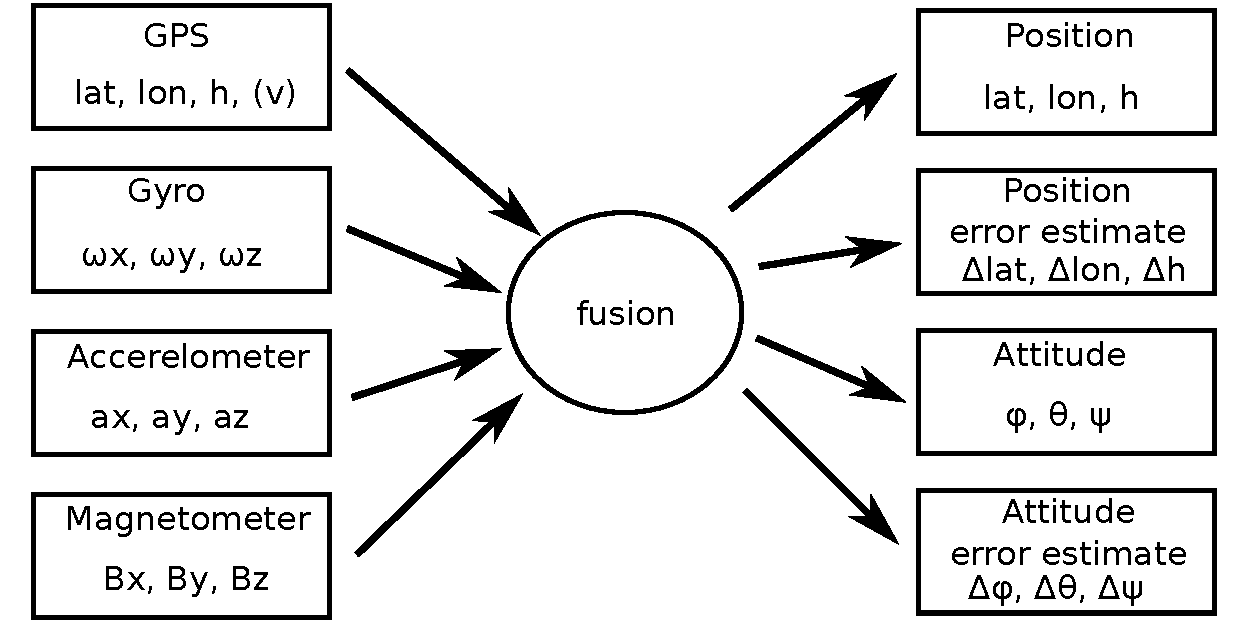
\includegraphics[width=0.8\textwidth]{figures/ADS_diagram.pdf}
\caption{Attitude Determination System overview}
\label{fig:ADS_overview}
\end{figure}

In order to produce high-accuracy attitude estimates and compensate for disadvantages of certain sensor types such as drift and noise, we chose to use a variety of sensors and fuse their information to a combined information.
The facilitated sensors will be (see figure \ref{fig:ADS_overview}):
\begin{itemize}
\item GPS receiver: Provides absolute position values, but has much high-frequency noise
\item Gyroscope: Provides accurate relative pointing direction, but has drift.
\item Accerelometer: Provides absoulte pointing relative to the horizon (gravity) and linear acceleration.
\item Magnetometer: Provides absolute pointing relative to the earth's magnetic field.
\end{itemize}

Combined all together, these sensors provide complete information about the module's attitude.
As a fusion method we will use well-understood algorithms, such as the extended Kalman filter.

The fused information will be updated in real-time and stored together with each image snapshot.

For development of the software, a simulation module is being written that feeds simulated measurement data into the fusion algorithm.
By this the performance can be quantified and development gets much faster than with waiting for actual measurement data. 

The fusion algorithm being developed and implemented in C++ will use a Kalman-like approach with least-square estimators for an optimized estimation of position and attitude combined.
In a first simpler appoach, we treat position and attitude independetly, which is less accurate but more robust as the system is being developed.

\FloatBarrier
\section{Electrical Circuits}

As compared to the BeagleBone the delivered BeagleBoard's voltage at the pins
of the expansion header is only between 0~V and 1.8~V but the expected voltage
at the supply and the I2C interface for the sensors is 3.3~V additionally to
the external pull-up resistors on the I2C interface also voltage level
converters have to be used.
\\
\\
\textit{More information will be included in the final version...}